\subsection{The Automatic Quality User Story Artisan (AQUSA)} \label{usq_4}
The QUS framework provides guidelines for improving the quality of USs. To support the framework, Lucassen et al. propose the AQUSA tool, which exposes defects and deviations from good user story practice \cite{lucassen2016improving}. AQUSA primarily targets easily describable and algorithmically determinable defects in the clerical part of requirements engineering, focusing on syntactic and some pragmatic criteria, while omitting semantic criteria that require a deep understanding of requirements' content \cite{lucassen2016improving}.
AQUSA consists of five main architectural components (Figure \ref{fig:aqusa}): linguistic parser, US base, analyzer, enhancer, and report generator.
\begin{figure}
\center
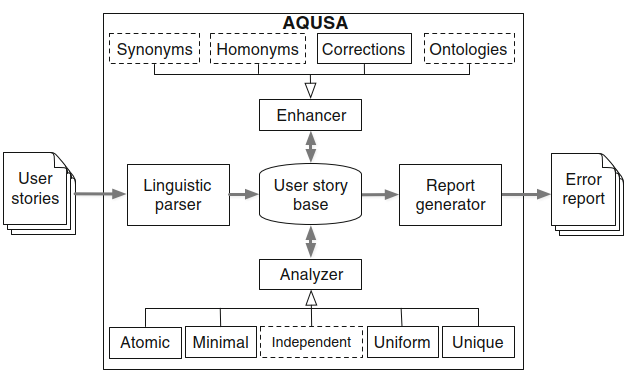
\includegraphics[width=13.03cm, height=7.76cm]{Functional_view_on_architecture_of_AQUSA}
\caption{Functional view on architecture of AQUSA. Dashed components are not fully implemented yet \cite{lucassen2016improving}}\label{fig:aqusa}
\end{figure} \\ 

The first step for every US is validating that it is well-formed. This takes place in the linguistic parser, which separates the user story in its role, means and end(s) parts. The US base captures the parsed US as an object according to the conceptual model, which acts as central storage.  Next, the analyzer runs tailormade method to verify specific syntactic and pragmatic quality criteria—where possible enhancers enrich the US base, improving the recall and precision of the analyzers. Finally, AQUSA captures the results in a comprehensive report \cite{lucassen2016improving}.

In the case of story analysis, AQUSA v1 conducts multiple analyses, beginning with the \emph{StoryChunker} and subsequently executing the Unique-, Minimal-, WellFormed-, Uniform-, and \emph{AtomicAnalyzer} modules. If any of these modules detect a violation of quality criteria, they engage the \emph{DefectGenerator} to record the defect in the associated database tables related to the story. Additionally, users have the option to utilize the AQUSA-GUI to access a project list or view a report of defects associated with a set of stories. \\ 
\textbf{Linguistic Parser: Well-Formed}\\ 
One of the essential aspects of verifying whether a string of text is a user story is splitting it into \emph{role}, \emph{means}, and \emph{end(s)}. This initial step is performed by the linguistic parser, implemented as the StoryChunker component. It identifies common indicators in the user story, such as \enquote{As a,} \enquote{I want to,} \enquote{I am able to,} and \enquote{so that.} The linguistic parser then categorizes words within each chunk using the Stanford NLP POS Tagger and validates the following rules for each chunk:
\begin{itemize}
\item Role: Checks if the last word is a noun representing an actor and if the words preceding the noun match a known role format (\emph{e.g.}, \enquote{as a}).
\item Means: Verifies if the first word is \enquote{I} and if a known means format like \enquote{want to} is present. It also ensures the remaining text contains at least one verb and one noun (\emph{e.g.}, \enquote{update event}).
\item End: Checks for the presence of an end and if it starts with a recognized end format (\emph{e.g.}, \enquote{so that}).
\end{itemize}
The linguistic parser validates whether a US adheres to the conceptual model. When it cannot detect a known means format, it retains the full user story and eliminates the role and end sections. If the remaining text contains both a verb and a noun, it's tagged as a \enquote{potential means,} and further analysis is conducted. Additionally, the parser checks for a comma after the role section. \\ 
\textbf{User Story Base and Enhancer}\\ 
Linguistically parsed USs are transformed into objects containing role, means, and ends components, aligning with the first level of decomposition in the conceptual model. These parsed USs are stored in the user story base for further processing. AQUSA enriches these USs by adding potential synonyms, homonyms, and relevant semantic information sourced from an ontology to the pertinent words within each chunk. Additionally, AQUSA includes a corrections' subpart, ensuring precise defect correction where possible. \\ 
\textbf{Analyzer: Explicit Dependencies}\\ 
AQUSA enforces that USs with explicit dependencies on other USs should include navigable links to those dependencies. It checks for numbers within USs and verifies whether these numbers are enclosed within links. For instance, if a US reads, \enquote{As a care professional, I want to edit the planned task I selected—see 908,} AQUSA suggests changing the isolated number to \enquote{See PID-908,} where PID represents the project identifier. When integrated with an issue tracker like Jira or Pivotal Tracker, this change would automatically generate a link to the dependency, such as \enquote{see PID-908 (\href{http://company.issuetracker.org/PID-908)}{http://company.issuetracker.org/PID-908}.} It's worth noting that this explicit dependency analyzer has not been implemented in AQUSA v1 to ensure its universal applicability across various issue trackers.\\ 
\textbf{Analyzer: Atomic}\\ 
AQUSA examines USs to ensure that the means section focuses on a single feature. To do this, it parses the means section for occurrences of the conjunctions \enquote{and, \&, +, or}. If AQUSA detects double feature requests in a US, it includes them in its report and suggests splitting the US into multiple ones. 
For example, a US like \enquote{As a User, I’m able to click a particular location from the map and thereby perform a search of landmarks associated with that latitude-longitude combination} would prompt a suggestion to split it into two USs: (1) \enquote{As a User, I want to click a location from the map} and (2) \enquote{As a User, I want to search landmarks associated with the lat-long combination of a location.}

AQUSA v1 verifies the role and means chunks for the presence of the conjunctions \enquote{and, \&, +, or}. If any of these conjunctions are found, AQUSA checks whether the text on both sides of the conjunction conforms to the QUS criteria for valid roles or means. Only if these criteria are met, AQUSA records the text following the conjunction as an atomicity violation. \\ 
\textbf{Analyzer: Minimal}\\ 
AQUSA assesses the minimality of USs by examining the role and means of sections extracted during chunking and \emph{well-formedness} verification. If AQUSA successfully extracts these sections, it checks for any additional text following specific punctuation marks such as dots, hyphens, semicolons, or other separators. For instance, in the US \enquote{As a care professional I want to see the registered hours of this week (split into products and activities). See: Mockup from Alice NOTE: First create the overview screen—Then add validations,} AQUSA would flag all text following the first dot (\enquote{.}) as non-minimal. Additionally, any text enclosed within parentheses is also marked as non-minimal.
AQUSA v1 employs two separate minimality checks using regular expressions. The first check searches for occurrences of special punctuation marks like \enquote{, -, ?, ., *.} and marks any text following them as a minimality violation. The second check identifies text enclosed in brackets such as \enquote{(), [], \{\}, \textless\textgreater} and records it as a minimality violation. \\ 
\textbf{Analyzer: Uniform}\\ 
AQUSA, in addition to its chunking process, identifies and extracts the format parts of USs and calculates their occurrences across all USs in a set. The most frequently occurring format is designated as the standard US format. Any US that deviates from this standard format is marked as non-compliant and included in the error report. For example, if the standard format is \enquote{I want to,} AQUSA will flag a US like \enquote{As a User, I am able to delete a landmark} as non-compliant because it does not follow the standard.
After the linguistic parser processes all USs in a set, AQUSA v1 initially identifies the most common US format by counting the occurrences of indicator phrases and selecting the most frequent one. Later, the uniformity analyzer calculates the edit distance between the format of each individual US chunk and the most common format for that chunk. If the edit distance exceeds a threshold of 3, AQUSA v1 records the entire story as a uniformity violation. This threshold ensures that minor differences, like \enquote{I am} versus \enquote{I'm,} do not trigger uniformity violations, while more significant differences in phrasing, such as \enquote{want} versus \enquote{can,} \enquote{need,} or \enquote{able,} do. \\ 
\textbf{Analyzer: Unique}\\ 
AQUSA has the capability to utilize various similarity measures, leveraging the WordNet lexical database to detect semantic similarity. For each verb and object found in the means or end of a US, AQUSA performs a WordNet::Similarity calculation with the corresponding verbs or objects from all other USs. These individual calculations are combined to produce a similarity degree for two USs. If this degree exceeds 90\%, AQUSA flags the USs as potential duplicates. \\ 
\textbf{AQUSA-GUI: report generator}\\ 
After AQUSA detects a violation in the linguistic parser or one of the analyzers, it promptly creates a defect record in the database, including details such as the defect type, a highlight of where the defect is located within the US, and its severity. AQUSA utilizes this data to generate a comprehensive report for the user.
The report begins with a dashboard that provides a quick overview of the US set's quality. It displays the total number of issues, categorized into defects and warnings, along with the count of perfect stories. Below the dashboard, all USs containing issues are listed, accompanied by their respective warnings and errors. An example is illustrated in figure \ref{fig:aqusa_report}.
\begin{figure}
\center
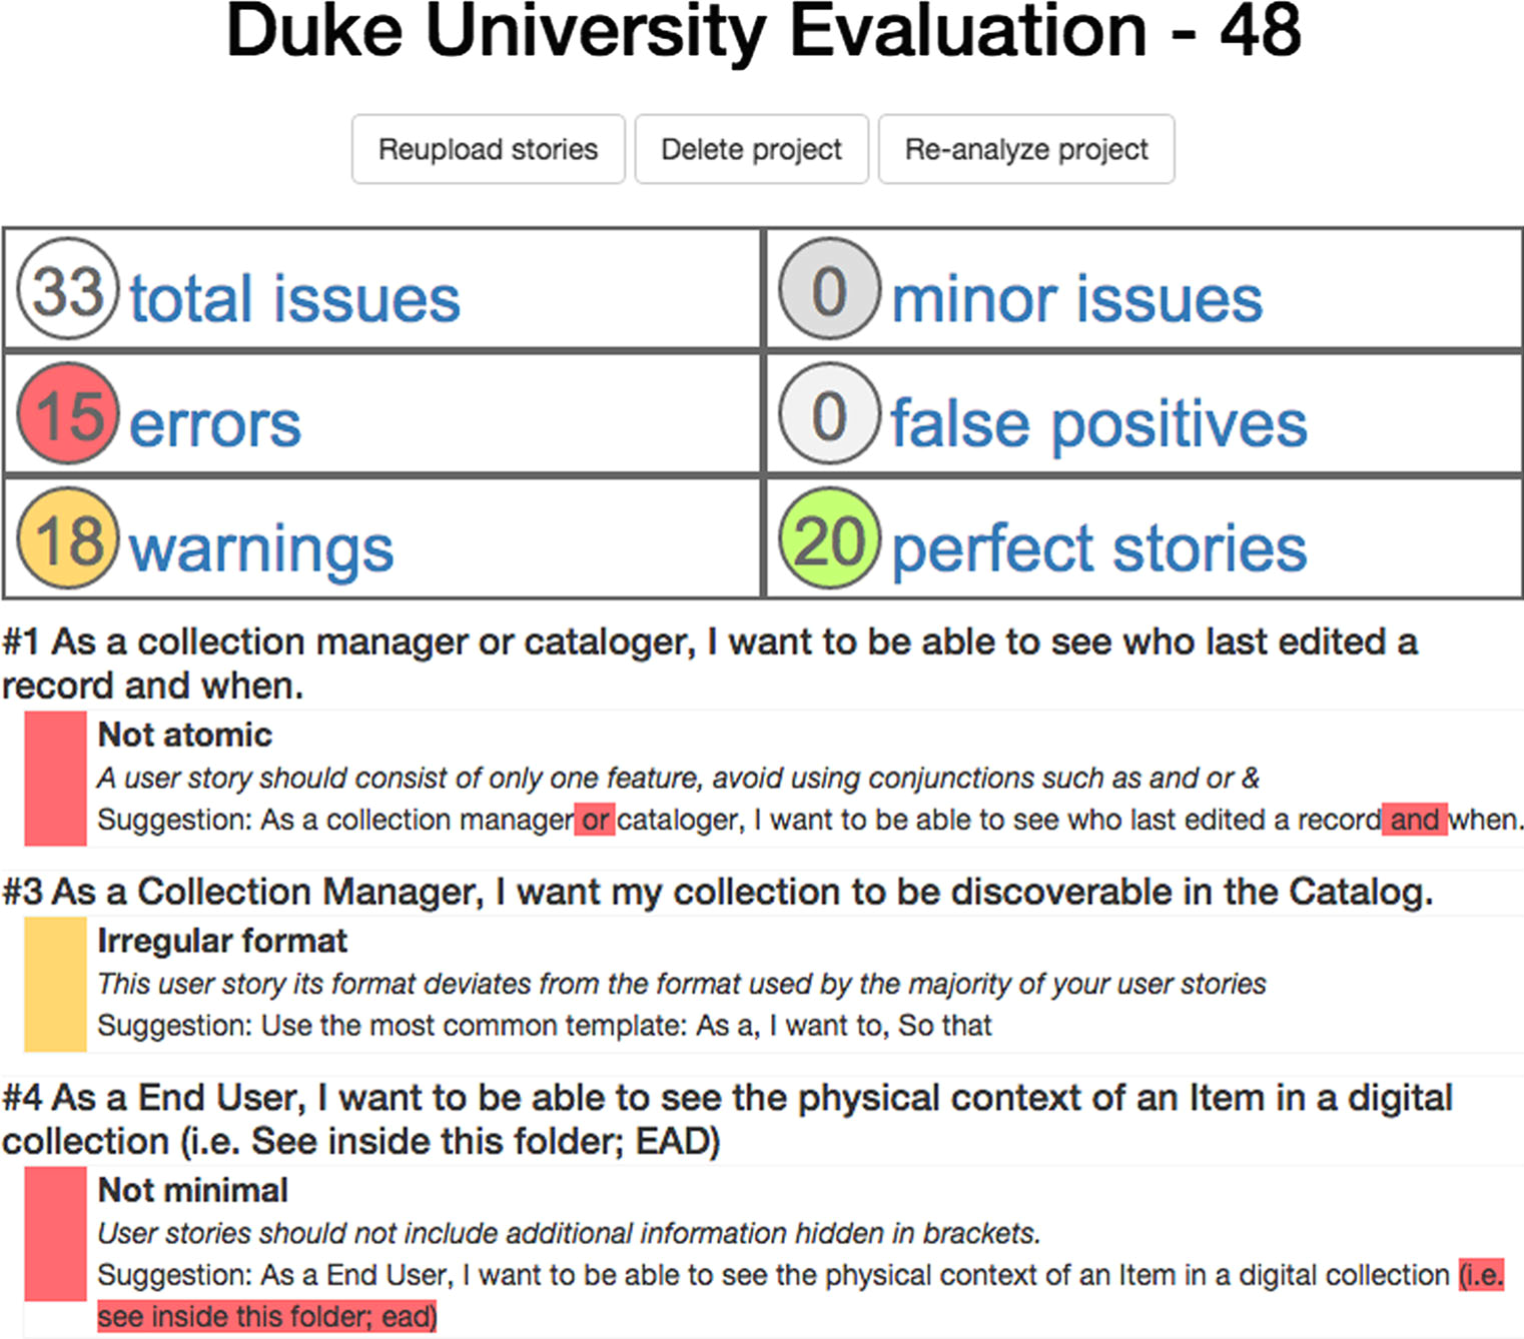
\includegraphics[width=11.03cm, height=9.76cm]{Example_report_of_a_defect_and_warning_for_a_story_in_AQUSA}
\caption{Example report of a defect and warning for a story in AQUSA \cite{lucassen2016improving}}\label{fig:aqusa_report}
\end{figure}
\subsection{Comparative Analysis} \label{usq_5}
In this subsection we consider a comparative analysis of mentioned methodologies to discern the most suitable approach for our specific context.
The IEEE Recommended Practice for Software Requirements Specifications defines requirements quality on the basis of eight characteristics \cite{doe2011recommended}: correct, unambiguous, complete, consistent, ranked for importance/stability, verifiable, modifiable, and traceable. The standard, however, is generic and it is well known that specifications are hardly able to meet those criteria \cite{glinz2000improving}. 

With agile requirements in mind, the Agile Requirements Verification Framework \cite{heck2014quality} defines three high-level verification criteria: completeness, uniformity, and consistency and correctness. The framework proposes specific criteria to be able to apply the quality framework to both feature requests and USs. Many of these criteria, however, require supplementary, unstructured information that is not captured in the primary US text. 

Quality frameworks often lack dedicated tools for tasks such as verifying unique IDs or establishing relationships between elements, making it necessary to rely on external tools like Jira for such checks.
Other sides the QUS Framework focuses on the intrinsic quality of the US text. Other approaches complement QUS by focusing on different notions of quality in RE quality such as performance with USs \cite{lombriser2016gamified} or broader requirements management concerns such as effort estimation and additional information sources such as descriptions or comments \cite{heck2014quality}. 
AQUSA, in conjunction with the QUS framework, is the only existed tools which offers several compelling reasons to consider its use for managing and enhancing USs in our approach: 

\begin{itemize}
\item \textbf{Conflict and Dependency between US:} The INVEST criteria's independence attribute effectively manages conflicts and dependencies among USs, ensuring that US do not overlap conceptually, allowing for flexible scheduling and implementation. 

Conversely, in a Quality framework, conflict and dependency between USs are regarded as conformance verification criteria, with a focus on ensuring that no two requirements or use cases are contradictory and that each requirement has a unique identifier. It's worth noting that the Quality framework does not encompass the verification of unique IDs or the establishment of relationships between elements; instead, third-party software is typically tasked with handling this. 

Within the Quality User Stories (QUS) framework, independence is emphasized as a pragmatic quality criterion, requiring that US be self-contained and devoid of inherent dependencies on other stories. Analyzing independencies through AQUSA v1 is a component of Lucassen et al. forthcoming efforts. They emphasis that is improbable that it will fully meet the Perfect Recall Condition unless a significant breakthrough in the computer’s comprehension of NLP emerges. This implies that the automated approach for analyzing conflicts and dependencies remains unresolved.
\item \textbf{Enhanced Quality Assurance:} AQUSA and the QUS framework provide a systematic approach to ensure the quality of USs. They help identify and rectify various defects, such as missing information, inconsistencies, and ambiguities, leading to more robust requirements.
\item \textbf{Defect Detection:} AQUSA automates the detection of defects within user stories, including well-formedness issues, uniqueness violations, minimal story violations, and more. This helps reduce the chances of miscommunication and misinterpretation among development teams.
\item \textbf{Efficient Workflow:} AQUSA streamlines the process of verifying USs, making it easier for requirements engineers and developers to focus on resolving issues rather than manually inspecting every story.
\item \textbf{Perfect Recall Condition:} AQUSA aims to fulfill the Perfect Recall Condition, minimizing the need for manual verification of USs. This can significantly reduce the risk of missed defects.
\item \textbf{Quality Assurance Across Tools:} AQUSA's ability to detect and highlight issues, adds an extra layer of quality assurance, helping ensure that USs in popular issue tracking tools like Jira and Pivotal Tracker are well-structured and coherent.
\item \textbf{Adaptability:} AQUSA can be customized to suit specific requirements and integrate with various issue tracking systems, making it adaptable to different development environments.
\item \textbf{Independence and Uniqueness:} AQUSA helps maintain the independence and uniqueness of USs, which is crucial for scheduling and implementing stories in any order without causing conflicts or overlaps.
\end{itemize}
\subsection{Conclusion} \label{usq_conclusion}
A closer look at the INVEST regarding dependencies and conflicts between USs, reveals that INVEST places great emphasis on promoting the autonomy of USs in order to dispense with their active management, which is mainly due to the complicated nature of such a management during the planning and prioritization phase. This perspective promotes a scenario in which USs can progress independently of the completion of other USs. Although this approach is undeniably idealistic, the pragmatic reality often deviates from this ideal. In practice, USs are often interdependent, so such linkages are almost inevitable. 

With regard to the quality framework, it can be seen that there are no explicit criteria relating to conflicts and dependencies between USs, but that it follows the INVEST criteria.

Moreover, it is worth noting that neither framework comes with built-in tools for the automatic analysis of USs. %Instead, they rely on third-party software such as Jira for this purpose.
The Quality Framework for User Stories (QUS) has a tool called AQUSA that automates the reporting of discrepancies in USs with respect to the QUS criteria. 

Analyzing dependencies through AQUSA v1 is a component of the forthcoming effort by Lucassen et al. Which means, the automatic analysis of dependencies and conflicts between USs is an area that requires future attention and development. In this context, we would like to contribute by addressing this unmet need.

















